\documentclass[]{article}
\usepackage{lmodern}
\usepackage{amssymb,amsmath}
\usepackage{ifxetex,ifluatex}
\usepackage{fixltx2e} % provides \textsubscript
\ifnum 0\ifxetex 1\fi\ifluatex 1\fi=0 % if pdftex
  \usepackage[T1]{fontenc}
  \usepackage[utf8]{inputenc}
\else % if luatex or xelatex
  \ifxetex
    \usepackage{mathspec}
  \else
    \usepackage{fontspec}
  \fi
  \defaultfontfeatures{Ligatures=TeX,Scale=MatchLowercase}
\fi
% use upquote if available, for straight quotes in verbatim environments
\IfFileExists{upquote.sty}{\usepackage{upquote}}{}
% use microtype if available
\IfFileExists{microtype.sty}{%
\usepackage{microtype}
\UseMicrotypeSet[protrusion]{basicmath} % disable protrusion for tt fonts
}{}
\usepackage[margin=1in]{geometry}
\usepackage{hyperref}
\hypersetup{unicode=true,
            pdftitle={Prediction Assignment},
            pdfauthor={Cynthia McGowan Poole},
            pdfborder={0 0 0},
            breaklinks=true}
\urlstyle{same}  % don't use monospace font for urls
\usepackage{color}
\usepackage{fancyvrb}
\newcommand{\VerbBar}{|}
\newcommand{\VERB}{\Verb[commandchars=\\\{\}]}
\DefineVerbatimEnvironment{Highlighting}{Verbatim}{commandchars=\\\{\}}
% Add ',fontsize=\small' for more characters per line
\usepackage{framed}
\definecolor{shadecolor}{RGB}{248,248,248}
\newenvironment{Shaded}{\begin{snugshade}}{\end{snugshade}}
\newcommand{\AlertTok}[1]{\textcolor[rgb]{0.94,0.16,0.16}{#1}}
\newcommand{\AnnotationTok}[1]{\textcolor[rgb]{0.56,0.35,0.01}{\textbf{\textit{#1}}}}
\newcommand{\AttributeTok}[1]{\textcolor[rgb]{0.77,0.63,0.00}{#1}}
\newcommand{\BaseNTok}[1]{\textcolor[rgb]{0.00,0.00,0.81}{#1}}
\newcommand{\BuiltInTok}[1]{#1}
\newcommand{\CharTok}[1]{\textcolor[rgb]{0.31,0.60,0.02}{#1}}
\newcommand{\CommentTok}[1]{\textcolor[rgb]{0.56,0.35,0.01}{\textit{#1}}}
\newcommand{\CommentVarTok}[1]{\textcolor[rgb]{0.56,0.35,0.01}{\textbf{\textit{#1}}}}
\newcommand{\ConstantTok}[1]{\textcolor[rgb]{0.00,0.00,0.00}{#1}}
\newcommand{\ControlFlowTok}[1]{\textcolor[rgb]{0.13,0.29,0.53}{\textbf{#1}}}
\newcommand{\DataTypeTok}[1]{\textcolor[rgb]{0.13,0.29,0.53}{#1}}
\newcommand{\DecValTok}[1]{\textcolor[rgb]{0.00,0.00,0.81}{#1}}
\newcommand{\DocumentationTok}[1]{\textcolor[rgb]{0.56,0.35,0.01}{\textbf{\textit{#1}}}}
\newcommand{\ErrorTok}[1]{\textcolor[rgb]{0.64,0.00,0.00}{\textbf{#1}}}
\newcommand{\ExtensionTok}[1]{#1}
\newcommand{\FloatTok}[1]{\textcolor[rgb]{0.00,0.00,0.81}{#1}}
\newcommand{\FunctionTok}[1]{\textcolor[rgb]{0.00,0.00,0.00}{#1}}
\newcommand{\ImportTok}[1]{#1}
\newcommand{\InformationTok}[1]{\textcolor[rgb]{0.56,0.35,0.01}{\textbf{\textit{#1}}}}
\newcommand{\KeywordTok}[1]{\textcolor[rgb]{0.13,0.29,0.53}{\textbf{#1}}}
\newcommand{\NormalTok}[1]{#1}
\newcommand{\OperatorTok}[1]{\textcolor[rgb]{0.81,0.36,0.00}{\textbf{#1}}}
\newcommand{\OtherTok}[1]{\textcolor[rgb]{0.56,0.35,0.01}{#1}}
\newcommand{\PreprocessorTok}[1]{\textcolor[rgb]{0.56,0.35,0.01}{\textit{#1}}}
\newcommand{\RegionMarkerTok}[1]{#1}
\newcommand{\SpecialCharTok}[1]{\textcolor[rgb]{0.00,0.00,0.00}{#1}}
\newcommand{\SpecialStringTok}[1]{\textcolor[rgb]{0.31,0.60,0.02}{#1}}
\newcommand{\StringTok}[1]{\textcolor[rgb]{0.31,0.60,0.02}{#1}}
\newcommand{\VariableTok}[1]{\textcolor[rgb]{0.00,0.00,0.00}{#1}}
\newcommand{\VerbatimStringTok}[1]{\textcolor[rgb]{0.31,0.60,0.02}{#1}}
\newcommand{\WarningTok}[1]{\textcolor[rgb]{0.56,0.35,0.01}{\textbf{\textit{#1}}}}
\usepackage{graphicx,grffile}
\makeatletter
\def\maxwidth{\ifdim\Gin@nat@width>\linewidth\linewidth\else\Gin@nat@width\fi}
\def\maxheight{\ifdim\Gin@nat@height>\textheight\textheight\else\Gin@nat@height\fi}
\makeatother
% Scale images if necessary, so that they will not overflow the page
% margins by default, and it is still possible to overwrite the defaults
% using explicit options in \includegraphics[width, height, ...]{}
\setkeys{Gin}{width=\maxwidth,height=\maxheight,keepaspectratio}
\IfFileExists{parskip.sty}{%
\usepackage{parskip}
}{% else
\setlength{\parindent}{0pt}
\setlength{\parskip}{6pt plus 2pt minus 1pt}
}
\setlength{\emergencystretch}{3em}  % prevent overfull lines
\providecommand{\tightlist}{%
  \setlength{\itemsep}{0pt}\setlength{\parskip}{0pt}}
\setcounter{secnumdepth}{0}
% Redefines (sub)paragraphs to behave more like sections
\ifx\paragraph\undefined\else
\let\oldparagraph\paragraph
\renewcommand{\paragraph}[1]{\oldparagraph{#1}\mbox{}}
\fi
\ifx\subparagraph\undefined\else
\let\oldsubparagraph\subparagraph
\renewcommand{\subparagraph}[1]{\oldsubparagraph{#1}\mbox{}}
\fi

%%% Use protect on footnotes to avoid problems with footnotes in titles
\let\rmarkdownfootnote\footnote%
\def\footnote{\protect\rmarkdownfootnote}

%%% Change title format to be more compact
\usepackage{titling}

% Create subtitle command for use in maketitle
\providecommand{\subtitle}[1]{
  \posttitle{
    \begin{center}\large#1\end{center}
    }
}

\setlength{\droptitle}{-2em}

  \title{Prediction Assignment}
    \pretitle{\vspace{\droptitle}\centering\huge}
  \posttitle{\par}
    \author{Cynthia McGowan Poole}
    \preauthor{\centering\large\emph}
  \postauthor{\par}
      \predate{\centering\large\emph}
  \postdate{\par}
    \date{9/14/2019}


\begin{document}
\maketitle

\hypertarget{overview}{%
\subsection{Overview}\label{overview}}

The goal of this project is to predict the manner in which the exercise
was performed, meaning predict the ``classe'' variable in the training
set by using any of the other variables to make the prediction. This
report describes how the model was built, how cross validation was used,
the expected output of sample error, and why certain choices were made.
This report also uses the prediction model to predict 20 different test
cases.

\begin{Shaded}
\begin{Highlighting}[]
\KeywordTok{library}\NormalTok{(caret)}
\KeywordTok{library}\NormalTok{(rpart)}
\KeywordTok{library}\NormalTok{(rpart.plot)}
\KeywordTok{library}\NormalTok{(rattle)}
\KeywordTok{library}\NormalTok{(ggplot2)}
\KeywordTok{library}\NormalTok{(ggpubr)}
\KeywordTok{theme_set}\NormalTok{(}\KeywordTok{theme_pubr}\NormalTok{())}
\KeywordTok{library}\NormalTok{(vcd)}
\KeywordTok{library}\NormalTok{(corrplot)}
\end{Highlighting}
\end{Shaded}

\hypertarget{getting-and-cleaning-the-data}{%
\subsection{Getting and Cleaning the
Data}\label{getting-and-cleaning-the-data}}

\begin{Shaded}
\begin{Highlighting}[]
\NormalTok{trainData <-}\StringTok{ }\KeywordTok{read.csv}\NormalTok{(}\KeywordTok{url}\NormalTok{(}\StringTok{"https://d396qusza40orc.cloudfront.net/predmachlearn/pml-training.csv"}\NormalTok{),}\DataTypeTok{header=}\OtherTok{TRUE}\NormalTok{,}\DataTypeTok{na.strings=}\KeywordTok{c}\NormalTok{(}\StringTok{"NA"}\NormalTok{,}\StringTok{"#DIV/0!"}\NormalTok{,}\StringTok{""}\NormalTok{))}
\KeywordTok{dim}\NormalTok{(trainData)}
\end{Highlighting}
\end{Shaded}

\begin{verbatim}
## [1] 19622   160
\end{verbatim}

\begin{Shaded}
\begin{Highlighting}[]
\NormalTok{testData <-}\StringTok{ }\KeywordTok{read.csv}\NormalTok{(}\KeywordTok{url}\NormalTok{(}\StringTok{"https://d396qusza40orc.cloudfront.net/predmachlearn/pml-testing.csv"}\NormalTok{),}\DataTypeTok{header=}\OtherTok{TRUE}\NormalTok{,}\DataTypeTok{na.strings=}\KeywordTok{c}\NormalTok{(}\StringTok{"NA"}\NormalTok{,}\StringTok{"#DIV/0!"}\NormalTok{,}\StringTok{""}\NormalTok{))}
\KeywordTok{dim}\NormalTok{(testData)}
\end{Highlighting}
\end{Shaded}

\begin{verbatim}
## [1]  20 160
\end{verbatim}

We can see that training data has 19622 observations and 160 variables.
Likewise, test data has 20 observations and 160 variables.

That is a lot of variables. We can reduce the variable count by removing
any variables from the training and test data that are mostly NA values.

\begin{Shaded}
\begin{Highlighting}[]
\NormalTok{NATrain <-}\StringTok{ }\KeywordTok{sapply}\NormalTok{(trainData, }\ControlFlowTok{function}\NormalTok{(x) }\KeywordTok{mean}\NormalTok{(}\KeywordTok{is.na}\NormalTok{(x))) }\OperatorTok{>}\StringTok{ }\FloatTok{0.95}
\NormalTok{trainClean <-}\StringTok{ }\NormalTok{trainData[, NATrain}\OperatorTok{==}\NormalTok{F]}

\KeywordTok{dim}\NormalTok{(trainClean)}
\end{Highlighting}
\end{Shaded}

\begin{verbatim}
## [1] 19622    60
\end{verbatim}

\begin{Shaded}
\begin{Highlighting}[]
\NormalTok{NATest <-}\StringTok{ }\KeywordTok{sapply}\NormalTok{(testData, }\ControlFlowTok{function}\NormalTok{(x) }\KeywordTok{mean}\NormalTok{(}\KeywordTok{is.na}\NormalTok{(x))) }\OperatorTok{>}\StringTok{ }\FloatTok{0.95}
\NormalTok{testClean <-}\StringTok{ }\NormalTok{testData[, NATest}\OperatorTok{==}\NormalTok{F]}

\KeywordTok{dim}\NormalTok{(testClean)}
\end{Highlighting}
\end{Shaded}

\begin{verbatim}
## [1] 20 60
\end{verbatim}

This gets us down to 60 variables. We can also remove any Variables that
have hardly any variation.

\begin{Shaded}
\begin{Highlighting}[]
\NormalTok{nzv <-}\StringTok{ }\KeywordTok{nearZeroVar}\NormalTok{(trainClean, }\DataTypeTok{saveMetrics=}\OtherTok{TRUE}\NormalTok{)}
\NormalTok{trainClean <-}\StringTok{ }\NormalTok{trainClean[,nzv}\OperatorTok{$}\NormalTok{nzv}\OperatorTok{==}\OtherTok{FALSE}\NormalTok{]}

\KeywordTok{dim}\NormalTok{(trainClean)}
\end{Highlighting}
\end{Shaded}

\begin{verbatim}
## [1] 19622    59
\end{verbatim}

\begin{Shaded}
\begin{Highlighting}[]
\NormalTok{nzv2 <-}\StringTok{ }\KeywordTok{nearZeroVar}\NormalTok{(testClean, }\DataTypeTok{saveMetrics=}\OtherTok{TRUE}\NormalTok{)}
\NormalTok{testClean <-}\StringTok{ }\NormalTok{testClean[,nzv2}\OperatorTok{$}\NormalTok{nzv}\OperatorTok{==}\OtherTok{FALSE}\NormalTok{]}

\KeywordTok{dim}\NormalTok{(testClean)}
\end{Highlighting}
\end{Shaded}

\begin{verbatim}
## [1] 20 59
\end{verbatim}

Lastly, we remove the first 5 identification variables that do not make
sense to use for predictors

\begin{Shaded}
\begin{Highlighting}[]
\NormalTok{trainClean <-}\StringTok{ }\NormalTok{trainClean[, }\OperatorTok{-}\NormalTok{(}\DecValTok{1}\OperatorTok{:}\DecValTok{5}\NormalTok{)]}
\NormalTok{testClean  <-}\StringTok{ }\NormalTok{testClean[, }\OperatorTok{-}\NormalTok{(}\DecValTok{1}\OperatorTok{:}\DecValTok{5}\NormalTok{)]}
\KeywordTok{dim}\NormalTok{(trainClean)}
\end{Highlighting}
\end{Shaded}

\begin{verbatim}
## [1] 19622    54
\end{verbatim}

\begin{Shaded}
\begin{Highlighting}[]
\KeywordTok{dim}\NormalTok{(testClean)}
\end{Highlighting}
\end{Shaded}

\begin{verbatim}
## [1] 20 54
\end{verbatim}

We have greatly reduced the number of variables. Now we are ready for
building and testing our models.

\hypertarget{data-analysis-for-model-selection}{%
\section{Data Analysis for Model
Selection}\label{data-analysis-for-model-selection}}

I already have Training and Test Data but I will need to have data for
validation too, so I will split my training data into two sets, one for
training and one for validation.

\begin{Shaded}
\begin{Highlighting}[]
\NormalTok{inTrain <-}\StringTok{ }\KeywordTok{createDataPartition}\NormalTok{(}\DataTypeTok{y=}\NormalTok{trainClean}\OperatorTok{$}\NormalTok{classe, }\DataTypeTok{p=}\FloatTok{0.7}\NormalTok{, }\DataTypeTok{list=}\OtherTok{FALSE}\NormalTok{)}
\NormalTok{train <-}\StringTok{ }\NormalTok{trainClean[inTrain, ]}
\NormalTok{valid <-}\StringTok{ }\NormalTok{trainClean[}\OperatorTok{-}\NormalTok{inTrain, ]}
\KeywordTok{dim}\NormalTok{(train)}
\end{Highlighting}
\end{Shaded}

\begin{verbatim}
## [1] 13737    54
\end{verbatim}

\begin{Shaded}
\begin{Highlighting}[]
\KeywordTok{dim}\NormalTok{(valid)}
\end{Highlighting}
\end{Shaded}

\begin{verbatim}
## [1] 5885   54
\end{verbatim}

\hypertarget{decision-tree-model-dt}{%
\subsection{Decision Tree Model (DT)}\label{decision-tree-model-dt}}

Now I can building the first model. I will start by training and fitting
a Model using a simple Decision Tree.

\begin{Shaded}
\begin{Highlighting}[]
\KeywordTok{set.seed}\NormalTok{(}\DecValTok{33333}\NormalTok{)}
\NormalTok{trainDT <-}\StringTok{ }\KeywordTok{rpart}\NormalTok{(classe }\OperatorTok{~}\StringTok{ }\NormalTok{., }\DataTypeTok{data=}\NormalTok{train, }\DataTypeTok{method=}\StringTok{"class"}\NormalTok{)}
\KeywordTok{fancyRpartPlot}\NormalTok{(trainDT)}
\end{Highlighting}
\end{Shaded}

\begin{verbatim}
## Warning: labs do not fit even at cex 0.15, there may be some overplotting
\end{verbatim}

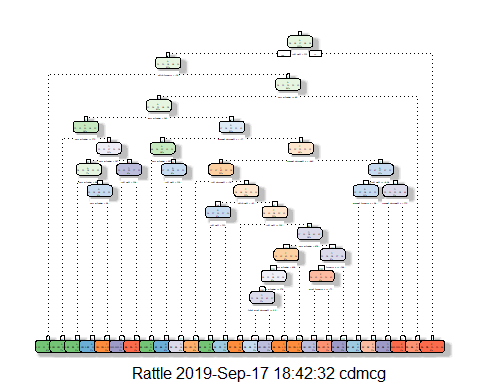
\includegraphics{predictionAssignment_files/figure-latex/train_DT-1.pdf}

Now we will run the DT model Predictions on the validation data

\begin{Shaded}
\begin{Highlighting}[]
\NormalTok{predictDT <-}\StringTok{ }\KeywordTok{predict}\NormalTok{(trainDT, }\DataTypeTok{newdata=}\NormalTok{valid, }\DataTypeTok{type=}\StringTok{"class"}\NormalTok{)}
\NormalTok{confMatrixDT <-}\StringTok{ }\KeywordTok{confusionMatrix}\NormalTok{(predictDT, valid}\OperatorTok{$}\NormalTok{classe)}
\NormalTok{confMatrixDT}
\end{Highlighting}
\end{Shaded}

\begin{verbatim}
## Confusion Matrix and Statistics
## 
##           Reference
## Prediction    A    B    C    D    E
##          A 1397   75    2    7    8
##          B  165  874   67   80   40
##          C    0   58  856   32    4
##          D   95   52   93  779   73
##          E   17   80    8   66  957
## 
## Overall Statistics
##                                           
##                Accuracy : 0.8263          
##                  95% CI : (0.8164, 0.8359)
##     No Information Rate : 0.2845          
##     P-Value [Acc > NIR] : < 2.2e-16       
##                                           
##                   Kappa : 0.7813          
##                                           
##  Mcnemar's Test P-Value : < 2.2e-16       
## 
## Statistics by Class:
## 
##                      Class: A Class: B Class: C Class: D Class: E
## Sensitivity            0.8345   0.7673   0.8343   0.8081   0.8845
## Specificity            0.9782   0.9258   0.9807   0.9364   0.9644
## Pos Pred Value         0.9382   0.7129   0.9011   0.7134   0.8484
## Neg Pred Value         0.9370   0.9431   0.9656   0.9614   0.9737
## Prevalence             0.2845   0.1935   0.1743   0.1638   0.1839
## Detection Rate         0.2374   0.1485   0.1455   0.1324   0.1626
## Detection Prevalence   0.2530   0.2083   0.1614   0.1856   0.1917
## Balanced Accuracy      0.9063   0.8466   0.9075   0.8722   0.9244
\end{verbatim}

Next we will plot the DT Model results

\begin{Shaded}
\begin{Highlighting}[]
\KeywordTok{mosaic}\NormalTok{(confMatrixDT}\OperatorTok{$}\NormalTok{table, }\DataTypeTok{shade =} \OtherTok{TRUE}\NormalTok{, }\DataTypeTok{legend =} \OtherTok{TRUE}\NormalTok{,}
                           \DataTypeTok{main =} \KeywordTok{paste}\NormalTok{(}\StringTok{"Decision Trees: Accuracy ="}\NormalTok{,}
                                        \KeywordTok{round}\NormalTok{(confMatrixDT}\OperatorTok{$}\NormalTok{overall[}\StringTok{'Accuracy'}\NormalTok{], }\DecValTok{4}\NormalTok{)))}
\end{Highlighting}
\end{Shaded}

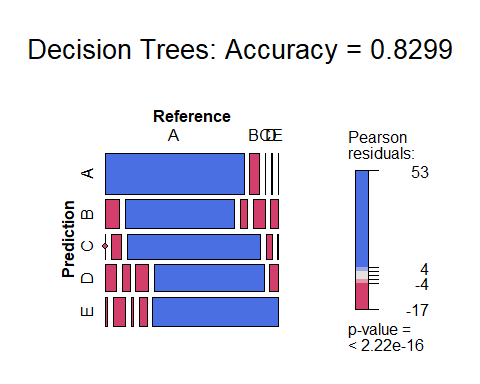
\includegraphics{predictionAssignment_files/figure-latex/plot_DT-1.pdf}

The accuracy of the DT model (0.8263) was not as good as I expected so
next I will fit a model using the gbm method. Decision trees are easy to
interpret but one drawback is that the results can vary greatly across
samples. I will try to increase the accuracy of the model by using a
boosting method.

\hypertarget{generalized-boosted-model-gbm}{%
\subsection{Generalized Boosted Model
(GBM)}\label{generalized-boosted-model-gbm}}

The GBM method builds upon the use of trees by splitting the sample into
multiple copies and fitting a separate tree to each copy, and then
applying the results of the current tree to the next tree thus training
the model slowly.

For this model I will use a training control to specify repeated cross
validation as the method to use for re-sampling. Using a training
control will give me some control over how robust the cross validation
will be.

\begin{Shaded}
\begin{Highlighting}[]
\KeywordTok{set.seed}\NormalTok{(}\DecValTok{33333}\NormalTok{)}
\NormalTok{controlGBM <-}\StringTok{ }\KeywordTok{trainControl}\NormalTok{(}\DataTypeTok{method =} \StringTok{"repeatedcv"}\NormalTok{, }\DataTypeTok{number =} \DecValTok{3}\NormalTok{, }\DataTypeTok{repeats =} \DecValTok{1}\NormalTok{)}
\NormalTok{trainGBM  <-}\StringTok{ }\KeywordTok{train}\NormalTok{(classe }\OperatorTok{~}\StringTok{ }\NormalTok{., }\DataTypeTok{data=}\NormalTok{train, }\DataTypeTok{method =} \StringTok{"gbm"}\NormalTok{,}
                    \DataTypeTok{trControl =}\NormalTok{ controlGBM, }\DataTypeTok{verbose =} \OtherTok{FALSE}\NormalTok{)}
\NormalTok{trainGBM}\OperatorTok{$}\NormalTok{finalModel}
\end{Highlighting}
\end{Shaded}

\begin{verbatim}
## A gradient boosted model with multinomial loss function.
## 150 iterations were performed.
## There were 53 predictors of which 53 had non-zero influence.
\end{verbatim}

Now we will run the GBM model Predictions on the validation data

\begin{Shaded}
\begin{Highlighting}[]
\NormalTok{predGBM <-}\StringTok{ }\KeywordTok{predict}\NormalTok{(trainGBM, }\DataTypeTok{newdata=}\NormalTok{valid)}
\NormalTok{confMatrixGBM <-}\StringTok{ }\KeywordTok{confusionMatrix}\NormalTok{(predGBM, valid}\OperatorTok{$}\NormalTok{classe)}
\NormalTok{confMatrixGBM}
\end{Highlighting}
\end{Shaded}

\begin{verbatim}
## Confusion Matrix and Statistics
## 
##           Reference
## Prediction    A    B    C    D    E
##          A 1672    7    0    0    0
##          B    2 1119    4    1    0
##          C    0   10 1020   16    4
##          D    0    2    2  945   20
##          E    0    1    0    2 1058
## 
## Overall Statistics
##                                           
##                Accuracy : 0.9879          
##                  95% CI : (0.9848, 0.9906)
##     No Information Rate : 0.2845          
##     P-Value [Acc > NIR] : < 2.2e-16       
##                                           
##                   Kappa : 0.9847          
##                                           
##  Mcnemar's Test P-Value : NA              
## 
## Statistics by Class:
## 
##                      Class: A Class: B Class: C Class: D Class: E
## Sensitivity            0.9988   0.9824   0.9942   0.9803   0.9778
## Specificity            0.9983   0.9985   0.9938   0.9951   0.9994
## Pos Pred Value         0.9958   0.9938   0.9714   0.9752   0.9972
## Neg Pred Value         0.9995   0.9958   0.9988   0.9961   0.9950
## Prevalence             0.2845   0.1935   0.1743   0.1638   0.1839
## Detection Rate         0.2841   0.1901   0.1733   0.1606   0.1798
## Detection Prevalence   0.2853   0.1913   0.1784   0.1647   0.1803
## Balanced Accuracy      0.9986   0.9905   0.9940   0.9877   0.9886
\end{verbatim}

Next we will plot the GBM Model results

\begin{Shaded}
\begin{Highlighting}[]
\KeywordTok{mosaic}\NormalTok{(confMatrixGBM}\OperatorTok{$}\NormalTok{table, }\DataTypeTok{shade =} \OtherTok{TRUE}\NormalTok{, }\DataTypeTok{legend =} \OtherTok{TRUE}\NormalTok{,}
                           \DataTypeTok{main =} \KeywordTok{paste}\NormalTok{(}\StringTok{"Generalized Boosted Mode: Accuracy ="}\NormalTok{,}
                                        \KeywordTok{round}\NormalTok{(confMatrixGBM}\OperatorTok{$}\NormalTok{overall[}\StringTok{'Accuracy'}\NormalTok{], }\DecValTok{4}\NormalTok{)))}
\end{Highlighting}
\end{Shaded}

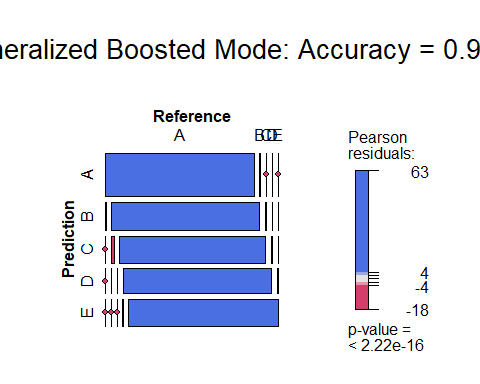
\includegraphics{predictionAssignment_files/figure-latex/plot_gbm-1.pdf}

The accuracy of the GBM model(0.9879) was much better than the DT Model
(0.8263 ). However, I will try one more model to see if I may get even
better accuracy.

\hypertarget{random-forest-model}{%
\subsection{Random Forest Model}\label{random-forest-model}}

For the last model, I will use the Random Forest method, which
re-samples using a random set of predictors to reduce the variance and
the error rate. I will again use a train control to specify repeated
cross validation as the method for re-sampling.

\begin{Shaded}
\begin{Highlighting}[]
\KeywordTok{set.seed}\NormalTok{(}\DecValTok{33333}\NormalTok{)}
\NormalTok{controlRF <-}\StringTok{ }\KeywordTok{trainControl}\NormalTok{(}\DataTypeTok{method=}\StringTok{"repeatedcv"}\NormalTok{, }\DataTypeTok{number=}\DecValTok{3}\NormalTok{, }\DataTypeTok{verboseIter=}\OtherTok{FALSE}\NormalTok{)}
\NormalTok{trainRF <-}\StringTok{ }\KeywordTok{train}\NormalTok{(classe }\OperatorTok{~}\StringTok{ }\NormalTok{., }\DataTypeTok{data=}\NormalTok{train, }\DataTypeTok{method=}\StringTok{"rf"}\NormalTok{,}
                          \DataTypeTok{trControl=}\NormalTok{controlRF)}
\NormalTok{trainRF}\OperatorTok{$}\NormalTok{finalModel}
\end{Highlighting}
\end{Shaded}

\begin{verbatim}
## 
## Call:
##  randomForest(x = x, y = y, mtry = param$mtry) 
##                Type of random forest: classification
##                      Number of trees: 500
## No. of variables tried at each split: 27
## 
##         OOB estimate of  error rate: 0.21%
## Confusion matrix:
##      A    B    C    D    E  class.error
## A 3905    0    0    0    1 0.0002560164
## B    4 2651    3    0    0 0.0026335591
## C    0    5 2391    0    0 0.0020868114
## D    0    0   11 2241    0 0.0048845471
## E    0    1    0    4 2520 0.0019801980
\end{verbatim}

Now we will run the Predictions on the validation data

\begin{Shaded}
\begin{Highlighting}[]
\CommentTok{# prediction on Test dataset}
\NormalTok{predRF <-}\StringTok{ }\KeywordTok{predict}\NormalTok{(trainRF, }\DataTypeTok{newdata=}\NormalTok{valid)}
\NormalTok{confMatrixRF <-}\StringTok{ }\KeywordTok{confusionMatrix}\NormalTok{(predRF, valid}\OperatorTok{$}\NormalTok{classe)}
\NormalTok{confMatrixRF}
\end{Highlighting}
\end{Shaded}

\begin{verbatim}
## Confusion Matrix and Statistics
## 
##           Reference
## Prediction    A    B    C    D    E
##          A 1673    0    0    0    0
##          B    1 1136    1    0    0
##          C    0    3 1025    3    0
##          D    0    0    0  961    6
##          E    0    0    0    0 1076
## 
## Overall Statistics
##                                          
##                Accuracy : 0.9976         
##                  95% CI : (0.996, 0.9987)
##     No Information Rate : 0.2845         
##     P-Value [Acc > NIR] : < 2.2e-16      
##                                          
##                   Kappa : 0.997          
##                                          
##  Mcnemar's Test P-Value : NA             
## 
## Statistics by Class:
## 
##                      Class: A Class: B Class: C Class: D Class: E
## Sensitivity            0.9994   0.9974   0.9990   0.9969   0.9945
## Specificity            1.0000   0.9996   0.9988   0.9988   1.0000
## Pos Pred Value         1.0000   0.9982   0.9942   0.9938   1.0000
## Neg Pred Value         0.9998   0.9994   0.9998   0.9994   0.9988
## Prevalence             0.2845   0.1935   0.1743   0.1638   0.1839
## Detection Rate         0.2843   0.1930   0.1742   0.1633   0.1828
## Detection Prevalence   0.2843   0.1934   0.1752   0.1643   0.1828
## Balanced Accuracy      0.9997   0.9985   0.9989   0.9978   0.9972
\end{verbatim}

Next we will plot the RF Model results

\begin{Shaded}
\begin{Highlighting}[]
\KeywordTok{mosaic}\NormalTok{(confMatrixRF}\OperatorTok{$}\NormalTok{table, }\DataTypeTok{shade =} \OtherTok{TRUE}\NormalTok{, }\DataTypeTok{legend =} \OtherTok{TRUE}\NormalTok{,}
                           \DataTypeTok{main =} \KeywordTok{paste}\NormalTok{(}\StringTok{"Random Forest: Accuracy ="}\NormalTok{,}
                                        \KeywordTok{round}\NormalTok{(confMatrixRF}\OperatorTok{$}\NormalTok{overall[}\StringTok{'Accuracy'}\NormalTok{], }\DecValTok{4}\NormalTok{))) }
\end{Highlighting}
\end{Shaded}

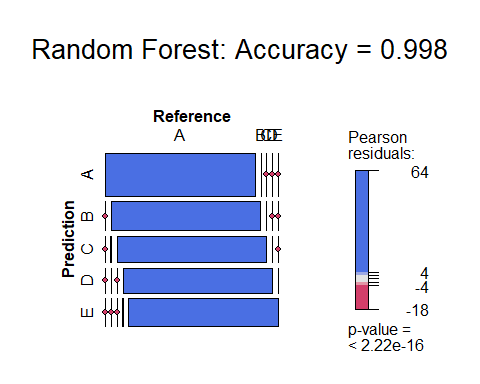
\includegraphics{predictionAssignment_files/figure-latex/plot_rf-1.pdf}

\#Model selection

\textbf{Summary of Results}\\
- Decision Trees: Accuracy = 0.8263\\
- Generalized Boosted Mode (GBM): Accuracy = 0.9879\\
- Random Forest (RF): Accuracy = 0.9976

From the results, it is clear that Random Forest is the best fit for the
data so I will fit the RF model to the full set of the training data to
get the best prediction against the actual test data.

\begin{Shaded}
\begin{Highlighting}[]
\NormalTok{trainFull <-}\StringTok{ }\NormalTok{trainClean}

\NormalTok{controlRF <-}\StringTok{ }\KeywordTok{trainControl}\NormalTok{(}\DataTypeTok{method=}\StringTok{"cv"}\NormalTok{, }\DataTypeTok{number=}\DecValTok{3}\NormalTok{, }\DataTypeTok{verboseIter=}\OtherTok{FALSE}\NormalTok{)}
\NormalTok{trainRF_Full <-}\StringTok{ }\KeywordTok{train}\NormalTok{(classe }\OperatorTok{~}\StringTok{ }\NormalTok{., }\DataTypeTok{data=}\NormalTok{trainFull, }\DataTypeTok{method=}\StringTok{"rf"}\NormalTok{,}
                          \DataTypeTok{trControl=}\NormalTok{controlRF)}
\NormalTok{trainRF_Full}\OperatorTok{$}\NormalTok{finalModel}
\end{Highlighting}
\end{Shaded}

\begin{verbatim}
## 
## Call:
##  randomForest(x = x, y = y, mtry = param$mtry) 
##                Type of random forest: classification
##                      Number of trees: 500
## No. of variables tried at each split: 27
## 
##         OOB estimate of  error rate: 0.14%
## Confusion matrix:
##      A    B    C    D    E  class.error
## A 5578    1    0    0    1 0.0003584229
## B    5 3789    2    1    0 0.0021069265
## C    0    5 3417    0    0 0.0014611338
## D    0    0   10 3205    1 0.0034203980
## E    0    0    0    1 3606 0.0002772387
\end{verbatim}

\hypertarget{getting-quiz-results-by-applying-the-model}{%
\subsection{Getting Quiz Results by Applying the
Model}\label{getting-quiz-results-by-applying-the-model}}

Lastly, I will apply the RF Model to the test data to predict the
answers to the 20 Test Cases.

\begin{Shaded}
\begin{Highlighting}[]
\NormalTok{testFull <-}\StringTok{ }\NormalTok{testClean}

\NormalTok{predictRF_Full <-}\StringTok{ }\KeywordTok{predict}\NormalTok{(trainRF_Full, }\DataTypeTok{newdata=}\NormalTok{testFull)}
\NormalTok{predictRF_Full}
\end{Highlighting}
\end{Shaded}

\begin{verbatim}
##  [1] B A B A A E D B A A B C B A E E A B B B
## Levels: A B C D E
\end{verbatim}


\end{document}
